\chapter{Análise de Resultados}
\label{cap:resultados}
Nesta capítulo são apresentados os resultados encontrados a partir dos três experimentos efetuados. Primeiro são apresentados os resultados encontrados  nos três experimentos, sendo assim feita uma análise da interferência nos mesmos. Em seguida é feita uma análise estatistica do experimento três sendo assim abordada, a questão da predição de desempenho.

\section{Interferência de Desempenho}
No primeiro experimento tinha como intuito, observar se de fato havia algum tipo de interferência significativa durante a execução de aplicações em máquinas virtuais concorrentes. Para isso, foram selecionadas as seguintes ferramentas: \textit{bzip2}, \textit{grep}, \textit{povray}, \textit{crypt} e \textit{cp} para calculo da degradação. A imagem \ref{first_experiment} apresenta os resultados para esse conjunto de aplicações inicial, utlizando a equação \ref{eq:combined}. 

\begin{figure}[!htb]
\centering
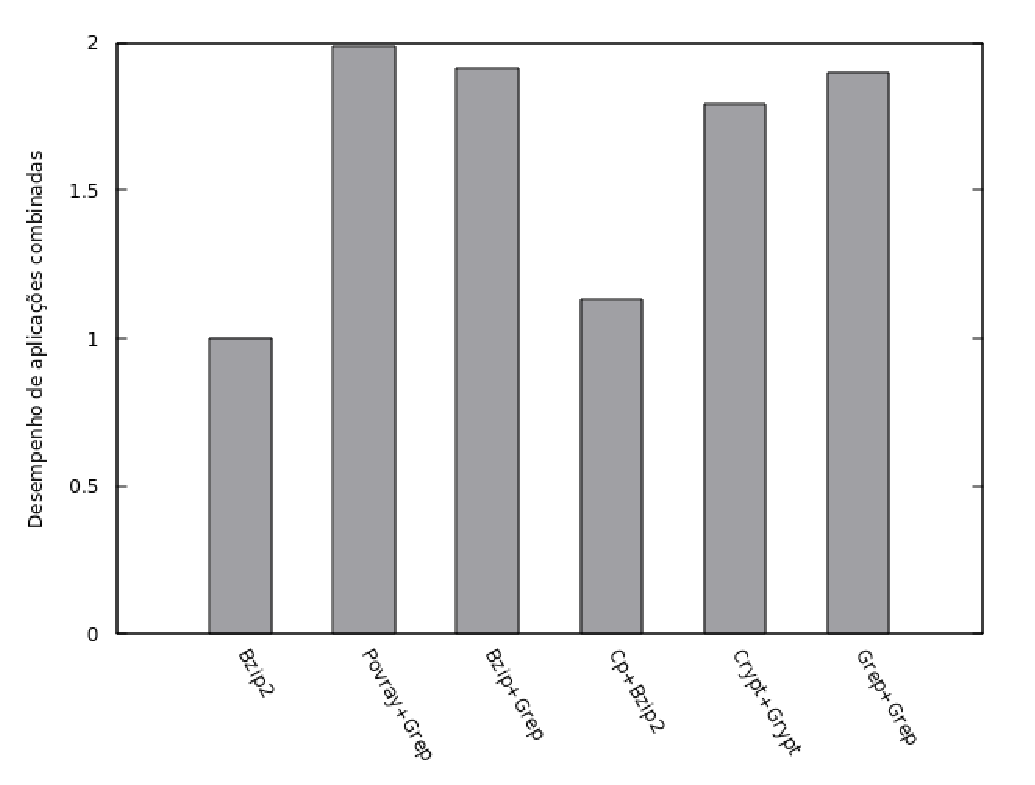
\includegraphics [keepaspectratio=true,scale=0.65]{graficos/exp1.eps}
\caption{Variação de desempenho para um conjunto de aplicações}
\label{first_experiment}
\end{figure} 

Levando-se em conta que cada aplicação consome exatamente metade dos recursos computacionais, o desempenho esperado seria 1. Entretanto, por conta da variação de interferência dada a combinação de aplicações, o desempenho também muda. Desse modo, aplicações que raramente interferem no desempenho uma da outra, a pontuação se a proxima de 2. Em contrapartida, aplicações que interferêm substancialmente uma na outra sua pontuação tende a cair drasticamente. Os resultados apresentados neste experimento, mostram por exemplo que \textit{povray+grep} apresentam um grau de interferência praticamente nulo, enquanto que \textit{cp + bzpip} o grau de interferência é maior a ponto da pontuação se aproximar de 1. Desse modo era de se esperar, que dado os resultados referentes a interferência de aplicações apresentados no trabalho de \citeonline{koh2007} que a performance combinada de aplicações iguais caisse drasticamente. Entretanto, os resultados de \textit{grep+grep} e \textit{crypt+crypt} mostram que mesmo aplicações iguais podem não interferir tanto quanto o esperado. Uma das hipóteses iniciais é de que configuração de disco em \textit{raid 5} do servidor, minimiza a interferência para aplicações com perfis de \textit{I\O} como \textit{Grep} e \textit{Crypt}.


%Análise da interferencia
%primeiro experimento
%segundo experimento
%Terceiro experimento
%características a nível de sistema
